\documentclass[a4paper, 11pt]{article}

% Nécessaire
\usepackage[french]{babel}
\usepackage[utf8]{inputenc}
\usepackage[T1]{fontenc}
\usepackage{lmodern}
\usepackage{amsmath, amsthm}
\usepackage{amsfonts,amssymb}

% Marge
\usepackage{geometry}
\geometry{margin={2.2cm ,2cm}}

% Figures, graphiques
\usepackage{graphicx}
\usepackage{epsfig}
\usepackage{caption}

% Surlignage
\usepackage{alltt}

\usepackage{xcolor}
\usepackage{soul}
\usepackage{color}
\usepackage{colortbl}

% Indicatrice
\usepackage{dsfont}

\usepackage{multirow}
\usepackage{eurosym}
\usepackage{extarrows}


% Titre
\title{Inflorescences}
\author{}
\date{}



\begin{document}
\maketitle

Ce document présente les différents jeux de données relatifs aux inflorescences qui seront utilisés ainsi que les modifications qui y ont étés apportées.
L'objectif est d'éditer des jeux de données correspondants non pas aux inflorescences vivantes mais aux inflorescences attractives. Sera déclarée attractive pour une inflorescence la période allant de sa date de débourrement jusqu'à $\Delta_t$ jours avant sa mort. Le $\Delta_t$ mentionné représente deux phénomènes différents : soit il représente le stade phénologique PF --- qui correspond à l'arrêt de l'élongation survenant avant la mort naturelle de l'inflorescence ---, soit il manifeste une période de déssechement (dûe à des attaques de cécidomyies) menant l'inflorescence à une mort certaine.

\section{Présentation des données}

Les données qui seront utilisées proviennent de deux jeux de données différents, avec des observations faites sur de la même parcelle.

\subsection{\textit{Dataset 1}}

Le \textit{dataset 1} contient des données relatives aux inflorescences, leurs dates de débourrements, de morts. Ont étés suivies entre le 19 juin et le 15 novembre 2017 deux cents unités de croissances (UCs). Pour chacune de ces UCs, un relevé régulier des inflorescences présentes a été effectué --- recensant leurs dates de débourrements et leurs dates de morts.
Il faut cependant noter que le relevé des dates de morts n'a commencé qu'à partir du 6 septembre.

De ce jeu de données on pourra obtenir les dates de débourrements et de morts, les dynamiques d'inflorescences vivantes pour les trois sous-blocs, la durée moyenne effective des inflorescences (et l'écart-type associé).

\subsection{\textit{Dataset 2}}

Le second jeu de données concerne le piégeage des larves. Les relevés ont eu lieu entre le 18 juillet et le 6 octobre 2017. Pour chacun des trois sous-blocs, dix arbres ont étés selectionnés aléatoirement sous lesquels ont été placés des pièges. À intervalle régulier furent comptées les larves piégées, les inflorescences au-dessus des pièges ainsi que le nombre d'inflorescences dans l'arbre.

\section{Théorie}

On commence par une simulation pour voir la différence attendue entre la dynamique d'inflorescences vivantes et la dynamique d'inflorescences attractives. Pour ce faire on simulera 1000 dates de débourrements suivant une gaussienne d'espérance 50 et d'écart-type 8.

On rajoutera 50 jours aux dates de débourrements pour avoir les inflorescences vivantes et 43 jour pour avoir les inflorescences attractives. Les résultats sont visibles sur la figure ci-dessous : 

\begin{figure}[h]
 \centering
 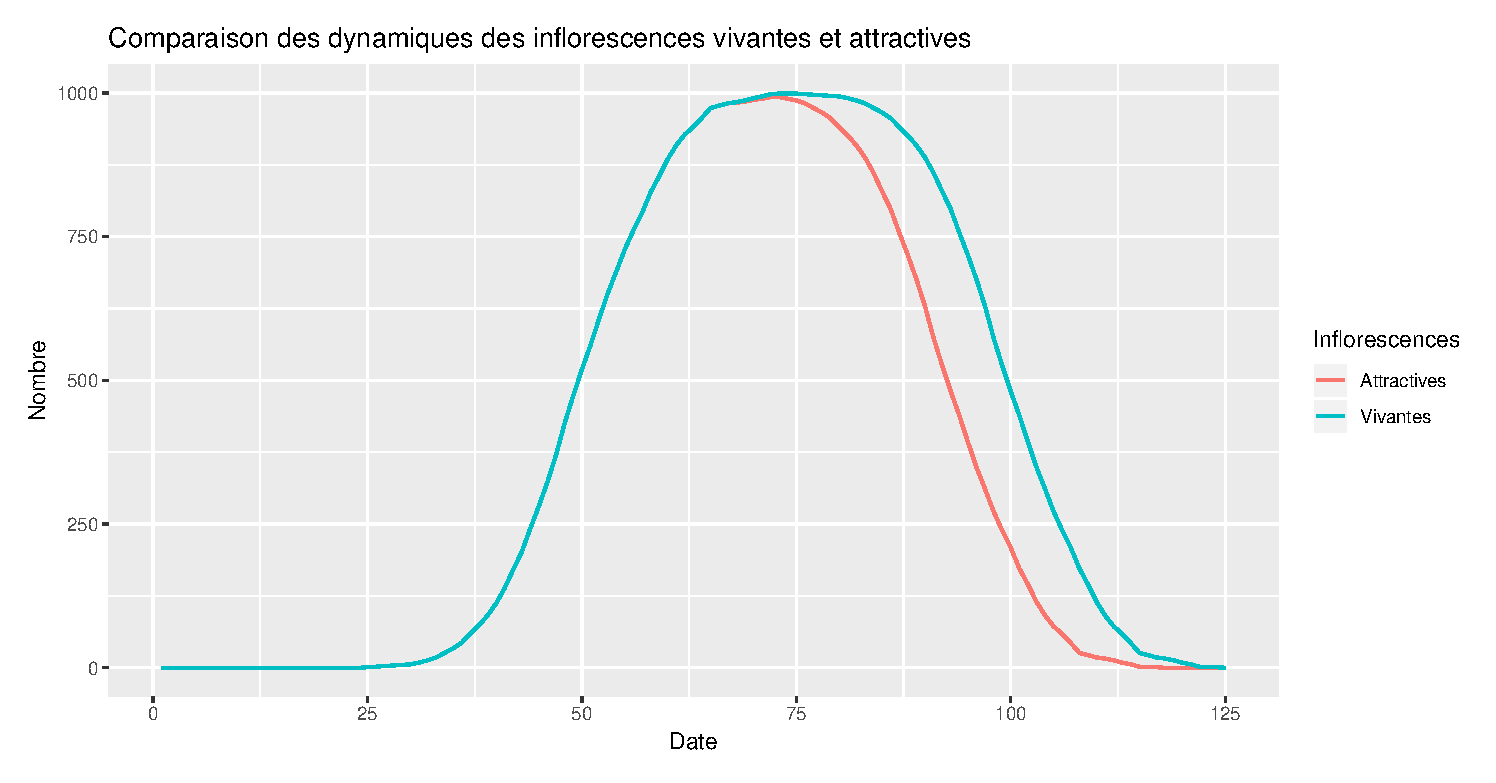
\epsfig{file = plots/comp.eps, scale = 0.65}
\end{figure}


On observe une dynamique similaire quoique légèrement moins intense, avec une moyenne apparaissant plus tôt et une dispersion moindre.

Un autre résultat notable : si l'on prend le vecteur comptabilisant le nombre de mort à chaque date, qu'on lui applique un décalage de 7 jours et que l'on recalcule les vivantes à partir de ce nouveau vecteur alors on retombe sur les inflorescences attractives.
Ce résultat sera utilisé par la suite.

\section{\textit{Dataset 1}}

Dans cette section, on décrira les modifications qui ont étés appliquées à la dynamique d'inflorescences issus du \textit{dataset 1} (comprenant les dates de débourrements et de morts des inflorescences) en vue d'avoir une dynamique d'inflorescences attractives.

La première modification apportée est une correction. En effet, sur ce jeu de données la distinction entre inflorescences vivantes et mortes n'a été faite qu'à partir du 6 septembre. Il en résulte un écart significatif dans la dynamique entre le 5 et 6 septembre. Cet écart correspond au nombre de mort qu'il y a eu avant le 6 septembre, qu'il faut donc répartir sur la période concernée. N'ayant aucune indication pour les répartir, on utilisera la dynamique d'inflorescences vivantes du \textit{dataset 2} (données relatives aux pièges) afin que la dynamique du \textit{dataset 1} ressemble le plus possible à la dynamique du \textit{dataset 2} à un coefficient de mise à l'échelle $\alpha$ près. Plus précisément, on attribuera un poids (à calibrer) pour tous les jours entre le jour 1 et le 5 septembre, et
le nombre de morts à chaque jour sera donné par la formule
$$M_t = \frac{p_t \times m}{\sum_j p_j},$$
où $M_t$ désigne le nombre de mort à la date $t$, $m$ le nombre de mort total déterminé par la différence d’inflorescences entre le 5 et 6 septembre et $p_t$ le poids assigné au jour $t$. Les poids $p_t$ et le coefficient de mise à l'échelle $\alpha$ seront déterminés par l'algorithme d'optimisation NSGA-II. Au niveau des notations, la dynamique issue du \textit{dataset 1} sera notée $I_t^1$, celle du \textit{dataset 2} sera notée $I_t^2$ et enfin celle du \textit{dataset 1} corrigée et mise à l'échelle sera notée $I_t^c$. Les résultats sont visibles ci-dessous pour les trois sous-blocs :

\begin{figure}[h]
 \centering
 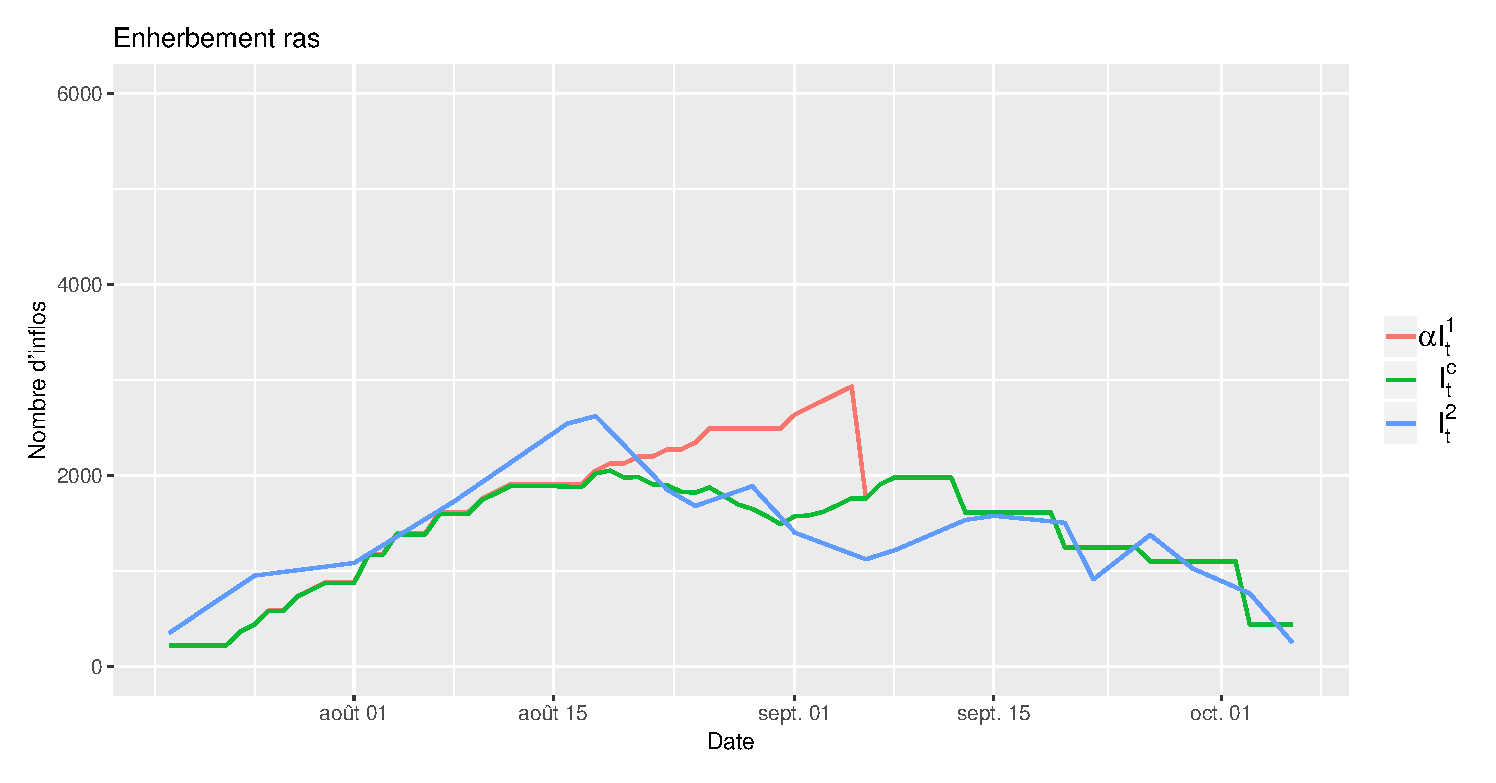
\epsfig{file = plots/corr_ER.eps, scale = 0.65}
\end{figure}
 
\begin{figure}[h]
 \centering
 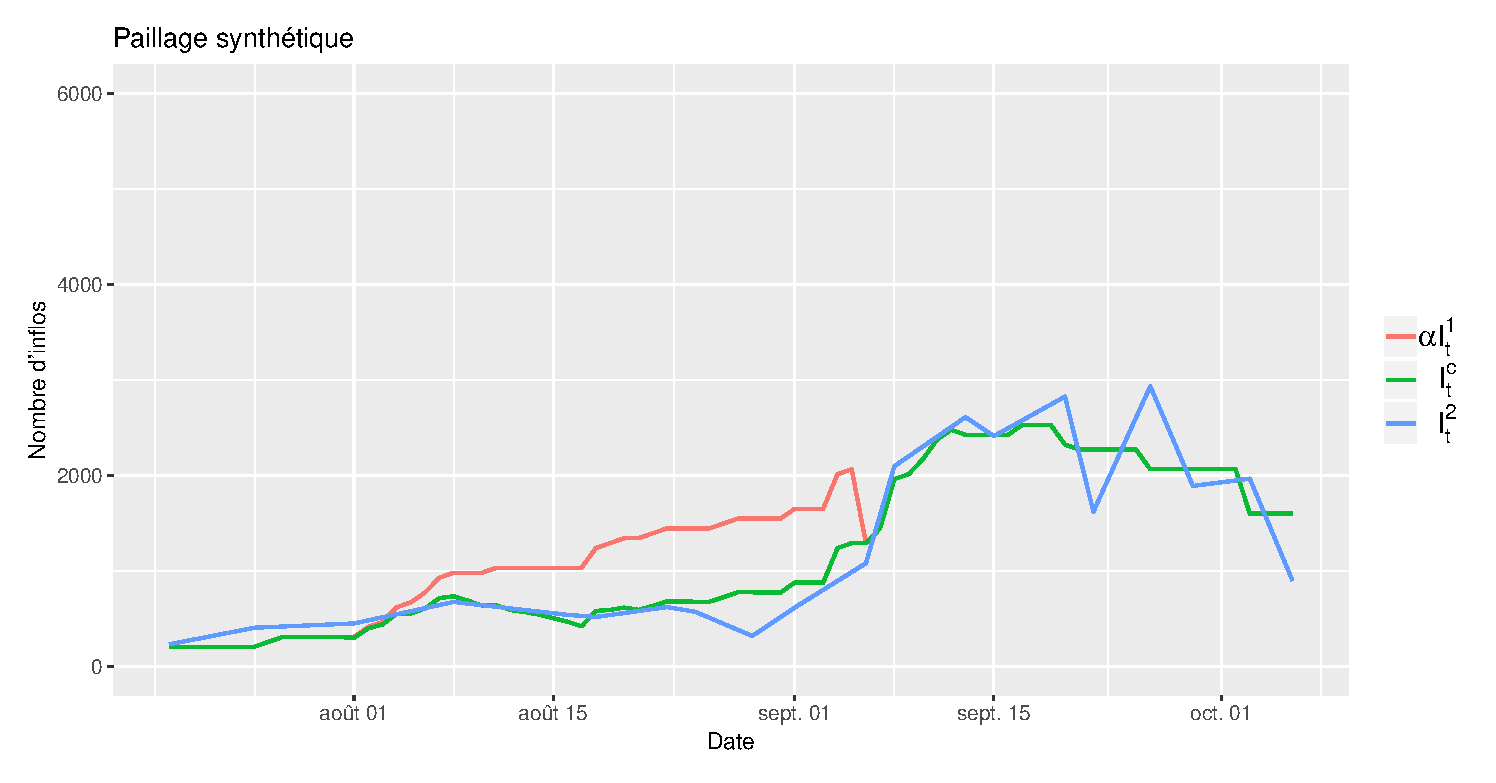
\epsfig{file = plots/corr_PS.eps, scale = 0.65}
\end{figure}

\begin{figure}[h]
 \centering
 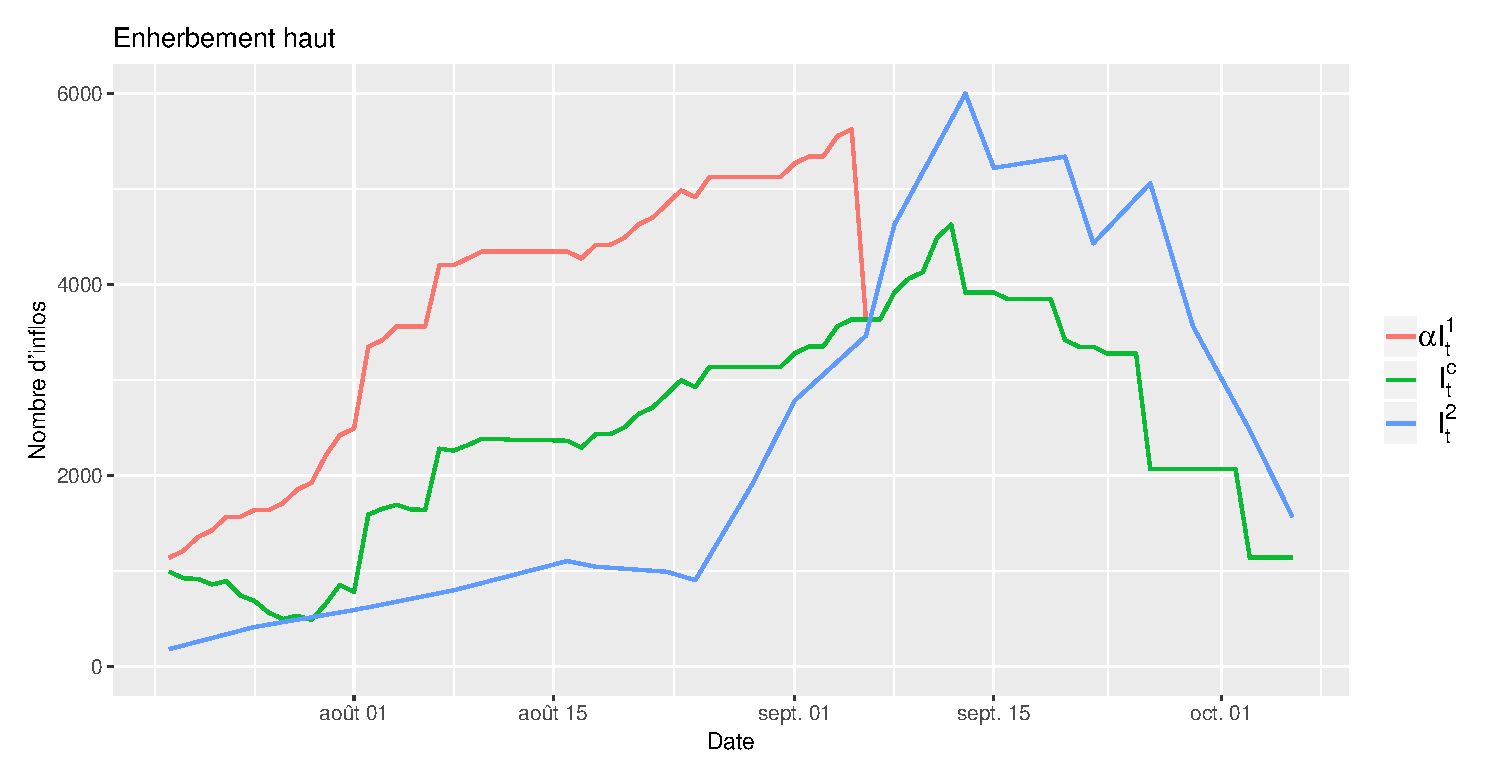
\epsfig{file = plots/corr_EH.eps, scale = 0.65}
\end{figure}

\clearpage

Pour introduire l'attractivité des inflorescences, il est nécessaire de récupérer --- pour chaque date --- le nombre de débourrements et le nombre d'inflorescences mortes. Pour les débourrements, on posera simplement $B_t^c = \alpha B_t^1$. Pour le nombre de mort (qui a été corrigé), cela se fait en deux étapes ; la première consiste à récupérer la somme cumulée des morts grâce à la formule
$$\sum_j^t B_j^c - I_t^c = \sum_j^t M_j,$$
et ensuite d'en déduire le nombre de mort quotidien $M_t$.

À partir de là, on peut décaler le vecteur des morts $M_t$ de 7 jours (comme vu en section 1) et obtenir ainsi la dynamique d'inflorescences attractives (qui sera noté $I_t^a$). Il faut noter qu'avec la correction effectuée précédemment, il y a des morts parmi les 7 premiers jours. Ces morts-là seront reportés sur les jours suivants.
Les différences entre $I_t^a$ et $I_t^c$, pour chacun des trois sous-blocs, sont visibles ci-dessous :

\begin{figure}[h]
 \centering
 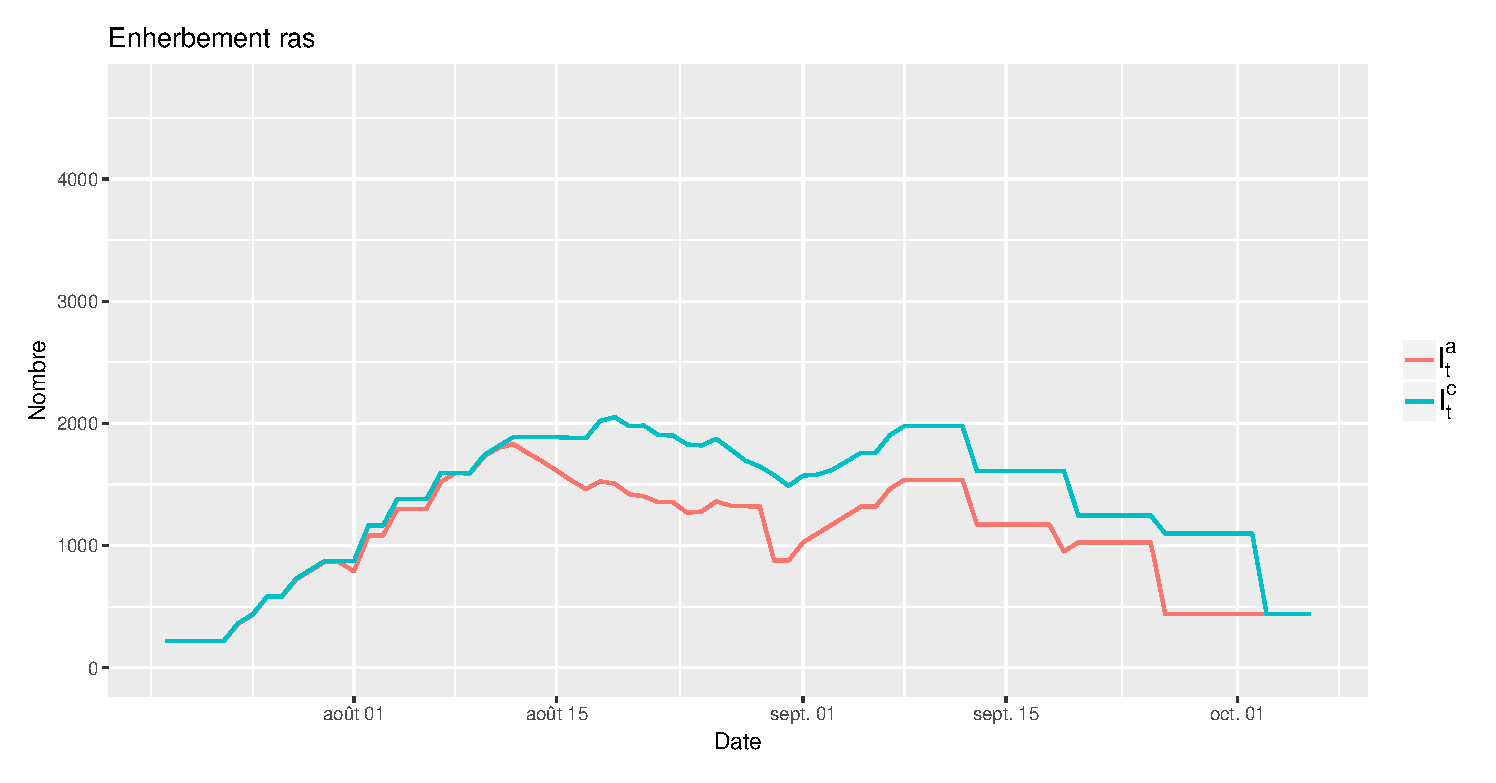
\epsfig{file = plots/attra_ER.eps, scale = 0.65}
\end{figure}
 
\begin{figure}[h]
 \centering
 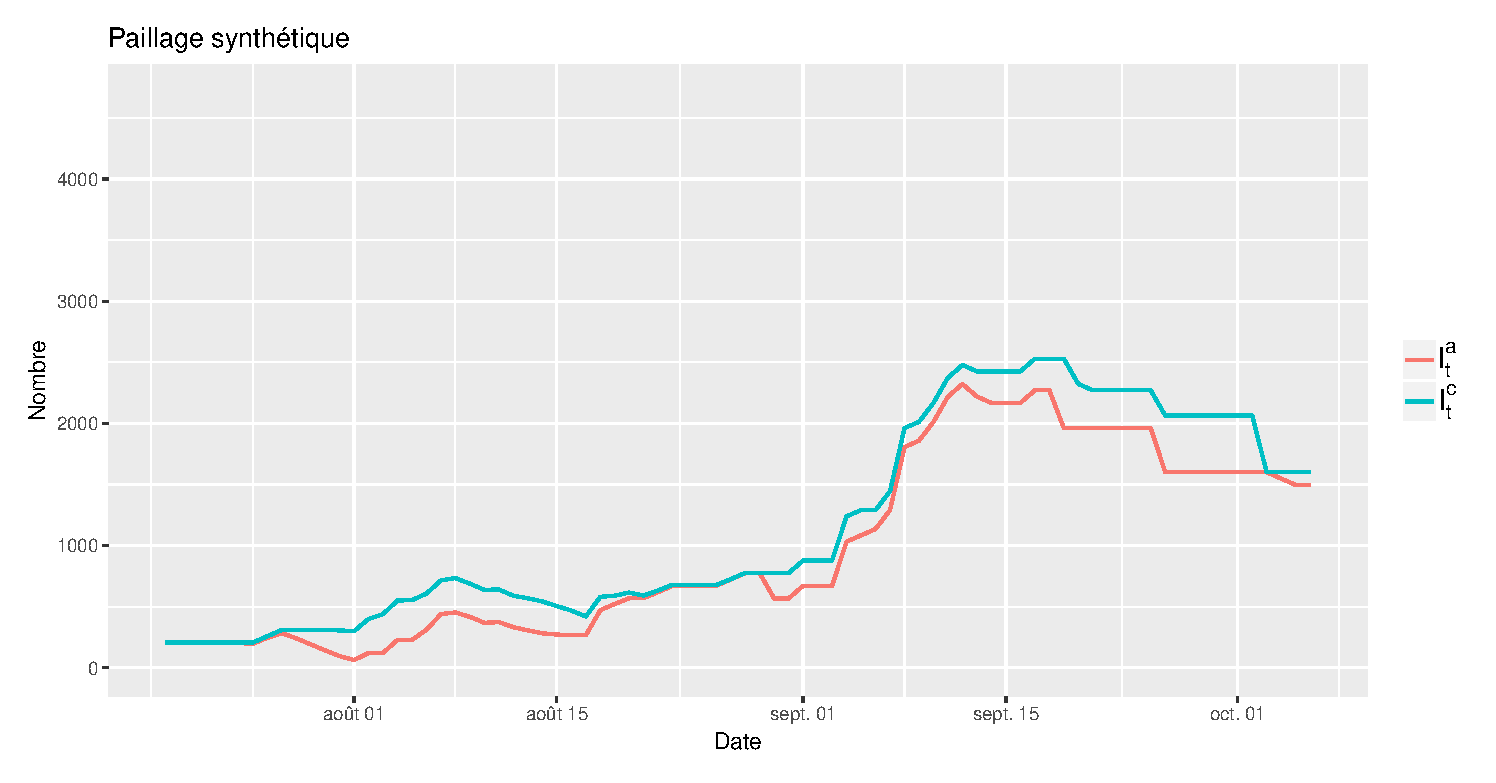
\epsfig{file = plots/attra_PS.eps, scale = 0.65}
\end{figure}

\begin{figure}[h]
 \centering
 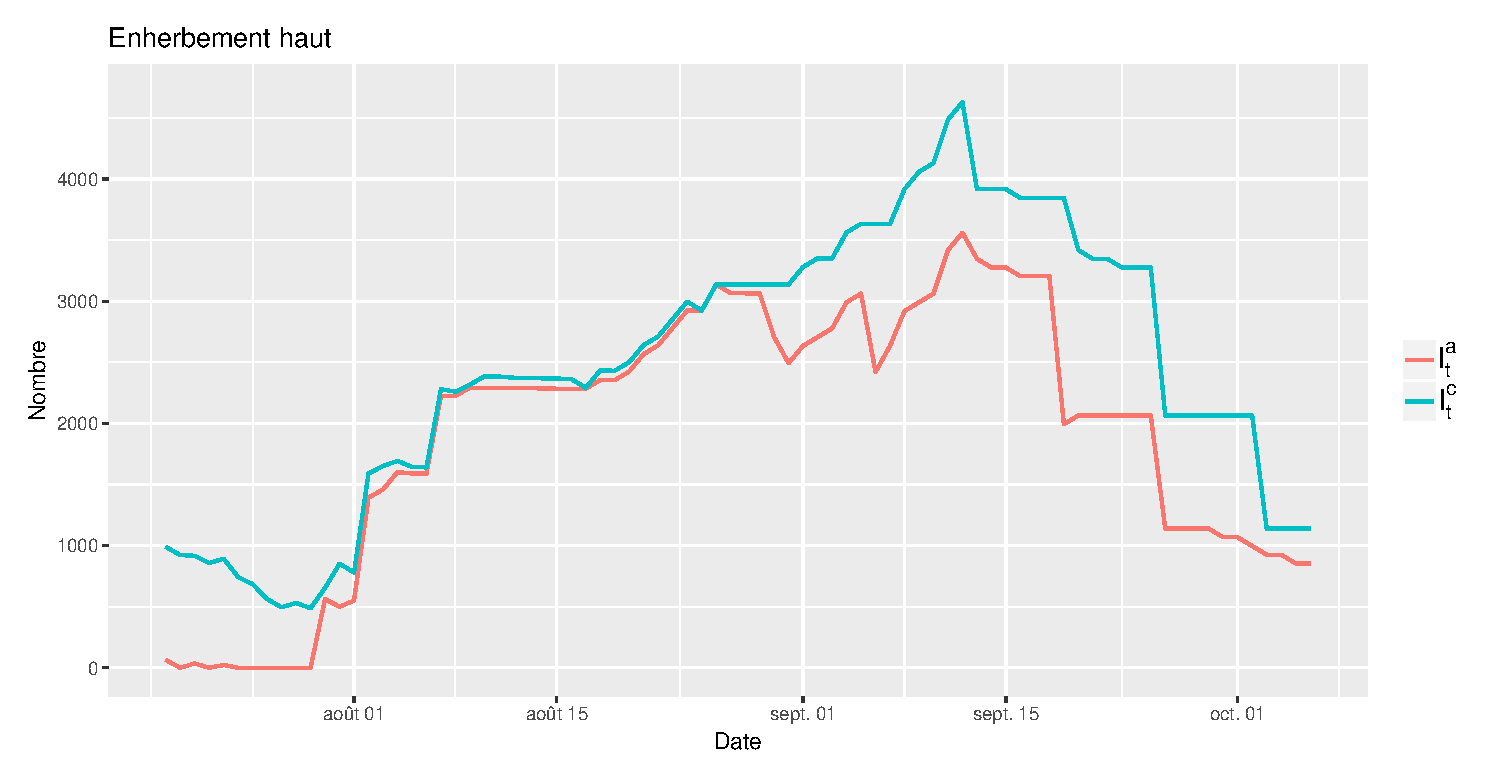
\epsfig{file = plots/attra_EH.eps, scale = 0.65}
\end{figure}


\section{Simulation de dynamiques d'inflorescences attractives}

Une deuxième approche a été testée : simuler les dates de débourrements pour coller au mieux aux inflorescences observées en utilisant la formule
$$I_t = B_t + \sum_{j = 1}^{50} B_{t-j}\times \left( 1 - F_{\mathcal{N}\left( 29, 14 \right)}(t-j) \right),$$
où 29 et 14 sont respectivement la moyenne et l’écart-type de la durée de vie des inflorescences observés sur le \textit{dataset 1}. On peut ensuite optimiser les date de débourrements pour coller au mieux à $I_t^2$, on notera $I_t^o$ les dynamiques obtenus.

Une fois les dates de débourrements obtenus, il devient possible de simuler une population d’inflorescences
attractives en utilisant la formule
$$I_t = B_t + \sum_{j = 1}^{50} B_{t-j}\times \left( 1 - F_{\mathcal{N}\left( 22, 14 \right)}(t-j) \right),$$
avec les $B_t$ déjà calibrés. Les dynamiques ainsi simulés seront notés $I_t^s$.

Par curiosité, on s'intéresse aussi à des inflorescences attractives où l'écart-type est fortement réduit (\textit{e.g.} à 2) simulées grâce à la formule
$$I_t = B_t + \sum_{j = 1}^{50} B_{t-j}\times \left( 1 - F_{\mathcal{N}\left( 22, 2 \right)}(t-j) \right).$$
On notera cette dynamique $I_t^{sd2}$.

Les résultats sont visibles ci-dessous :

\begin{figure}[!h]
 \centering
 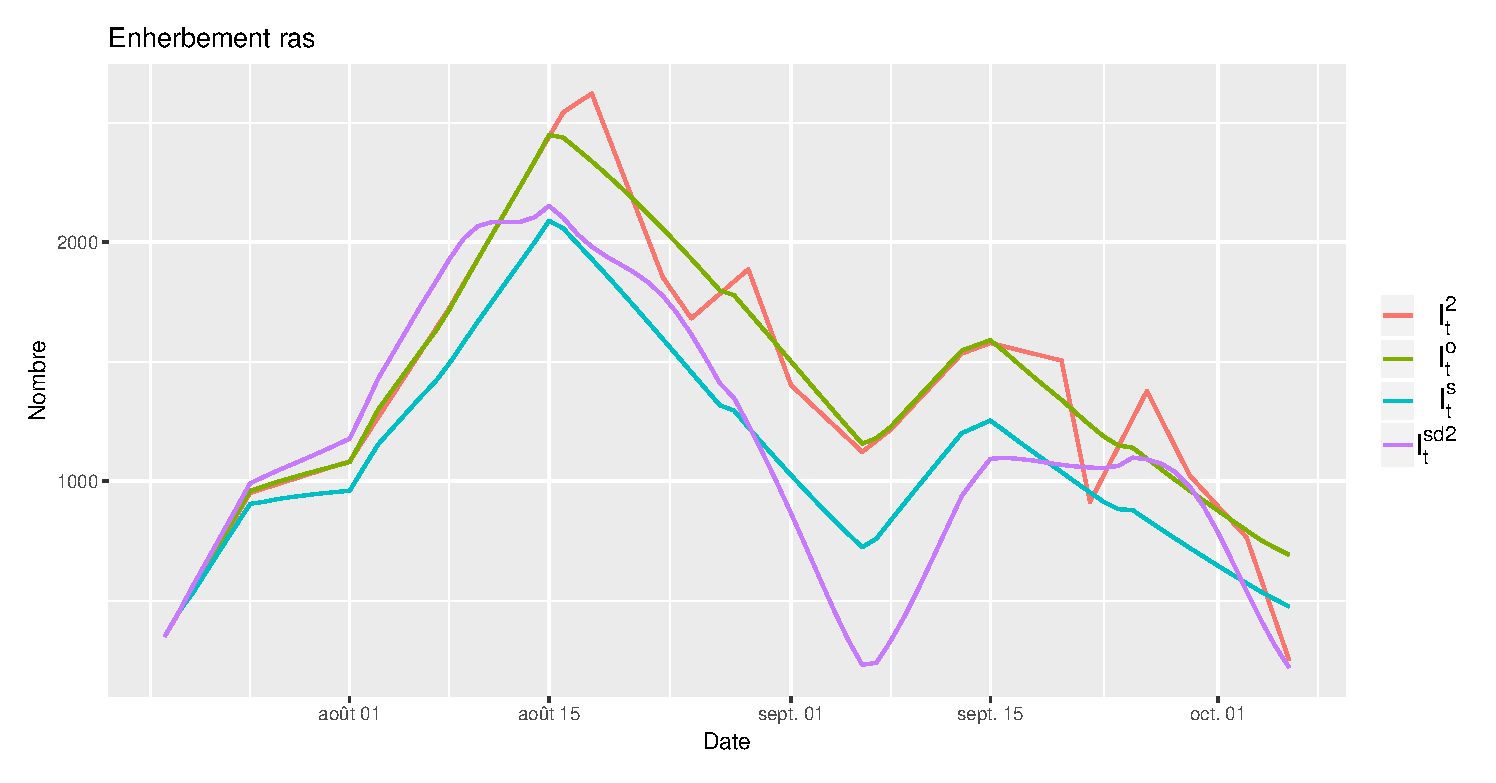
\epsfig{file = plots/sdmin_ER.eps, scale = 0.65}
\end{figure}
 
\begin{figure}[!h]
 \centering
 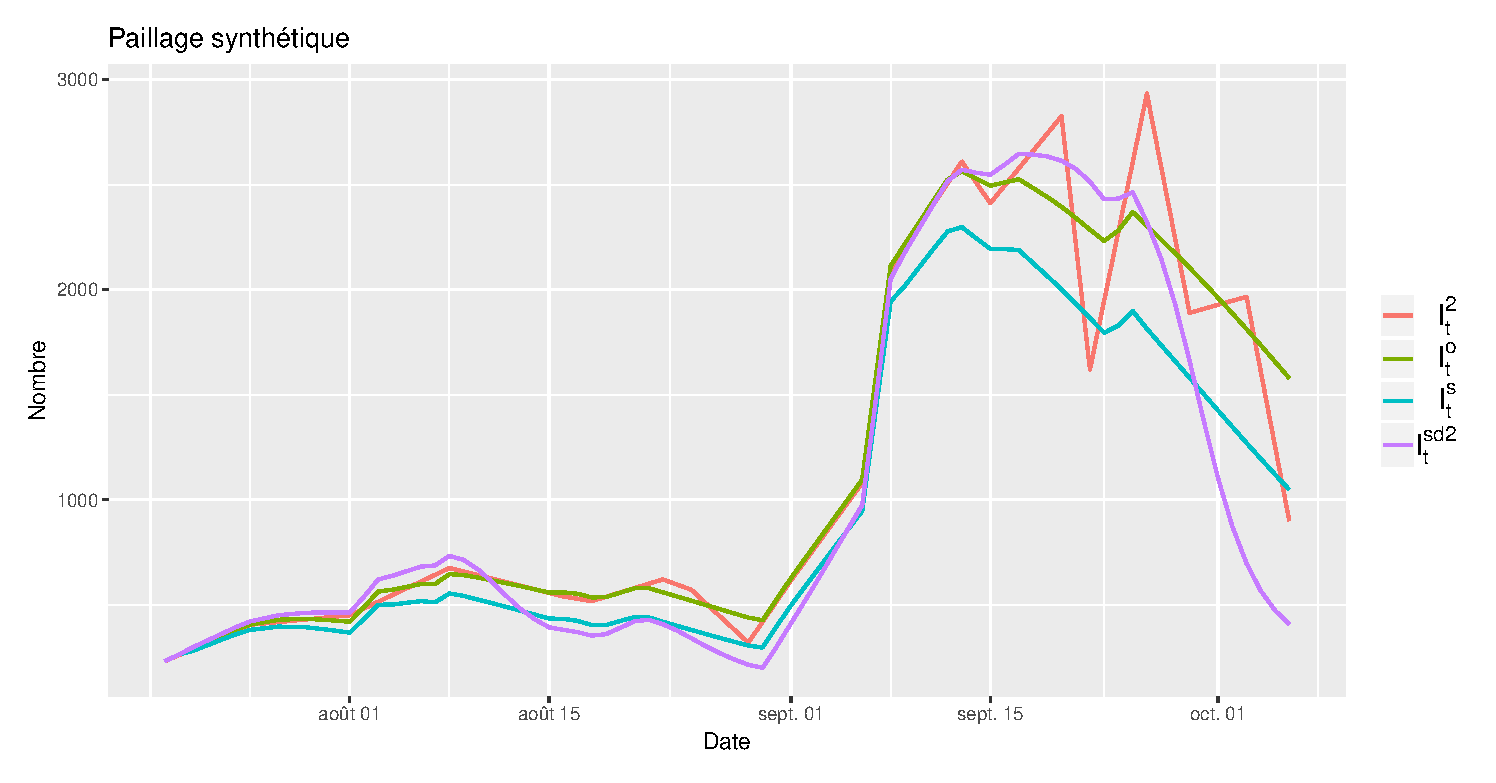
\epsfig{file = plots/sdmin_PS.eps, scale = 0.65}
\end{figure}

\begin{figure}[!h]
 \centering
 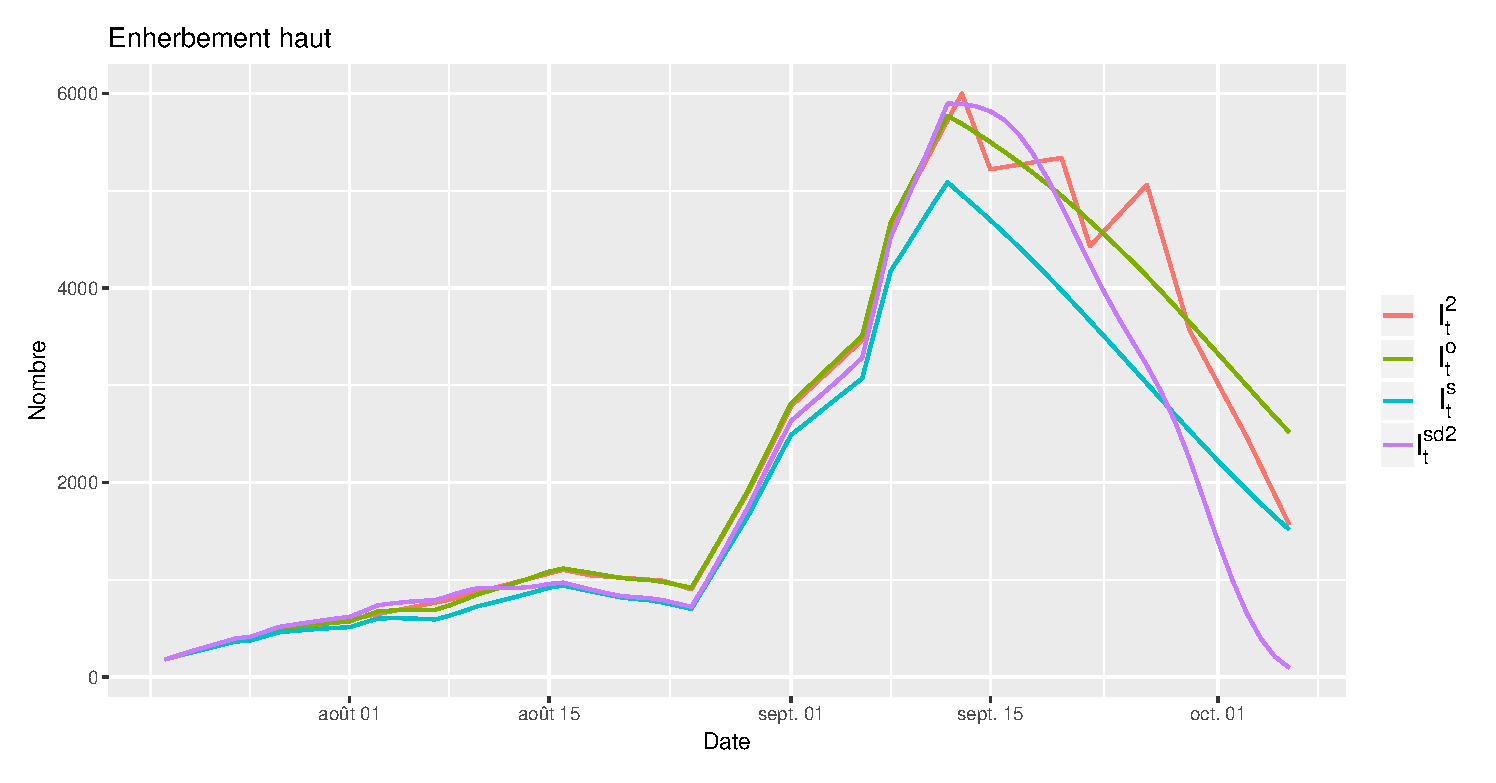
\epsfig{file = plots/sdmin_EH.eps, scale = 0.65}
\end{figure}

\clearpage


\section{Comparaison des deux approches}

Les graphes ci-dessous montrent la comparaison entre $I_t^a$ et $I_t^s$ qui seront utilisés comme entrée du sous-modèle 1.

\begin{figure}[h]
 \centering
 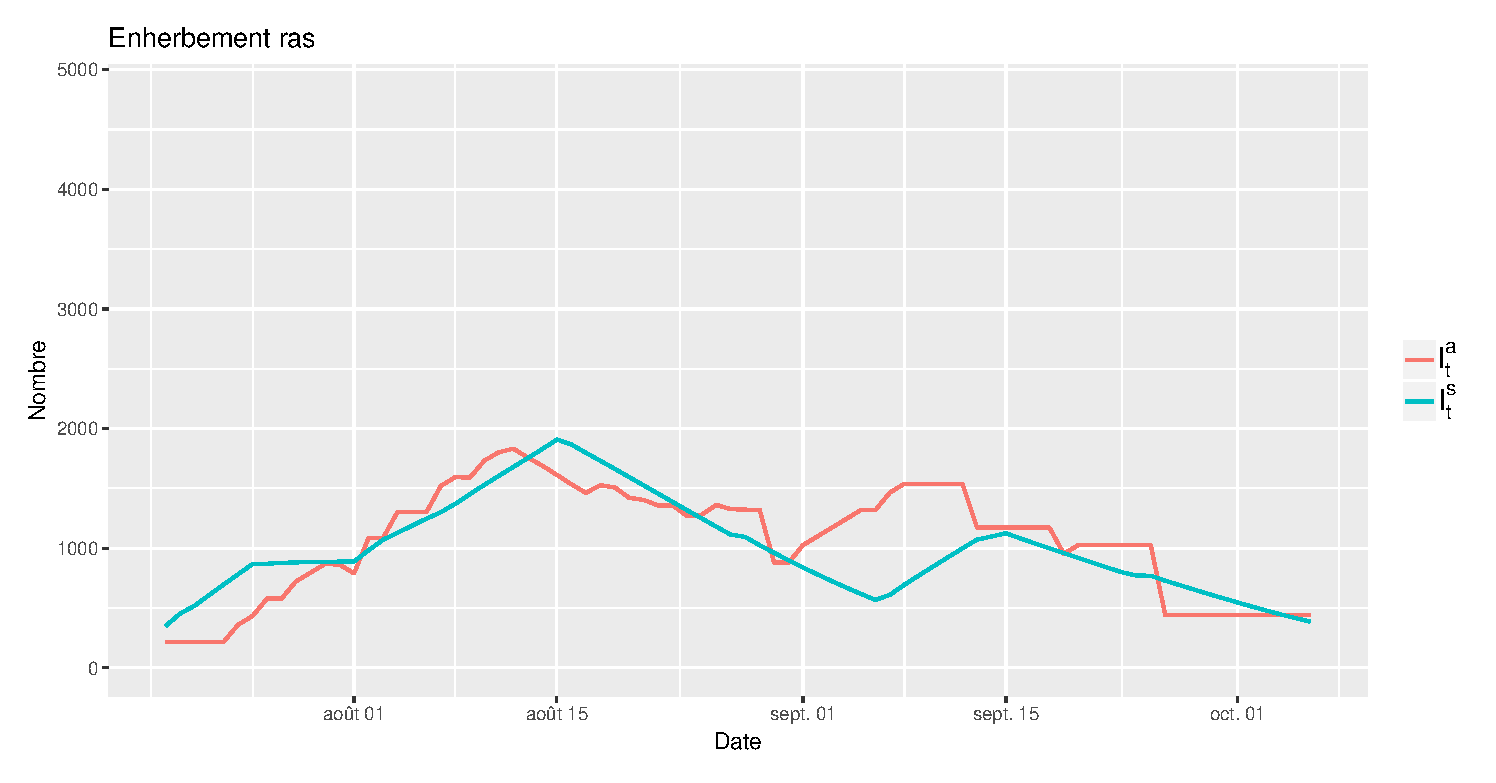
\epsfig{file = plots/comp_ER.eps, scale = 0.65}
\end{figure}
 
\begin{figure}[h]
 \centering
 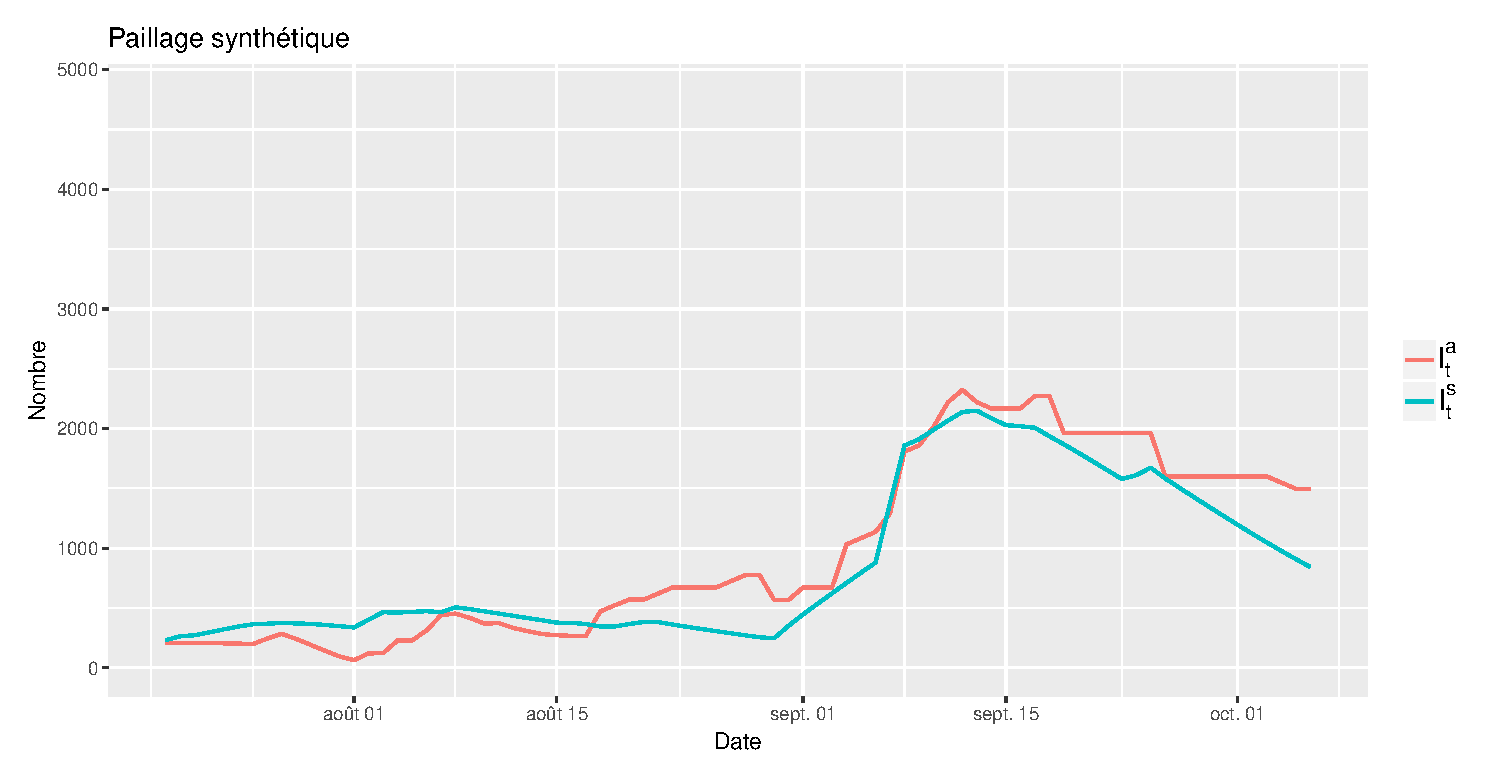
\epsfig{file = plots/comp_PS.eps, scale = 0.65}
\end{figure}

\begin{figure}[ht]
 \centering
 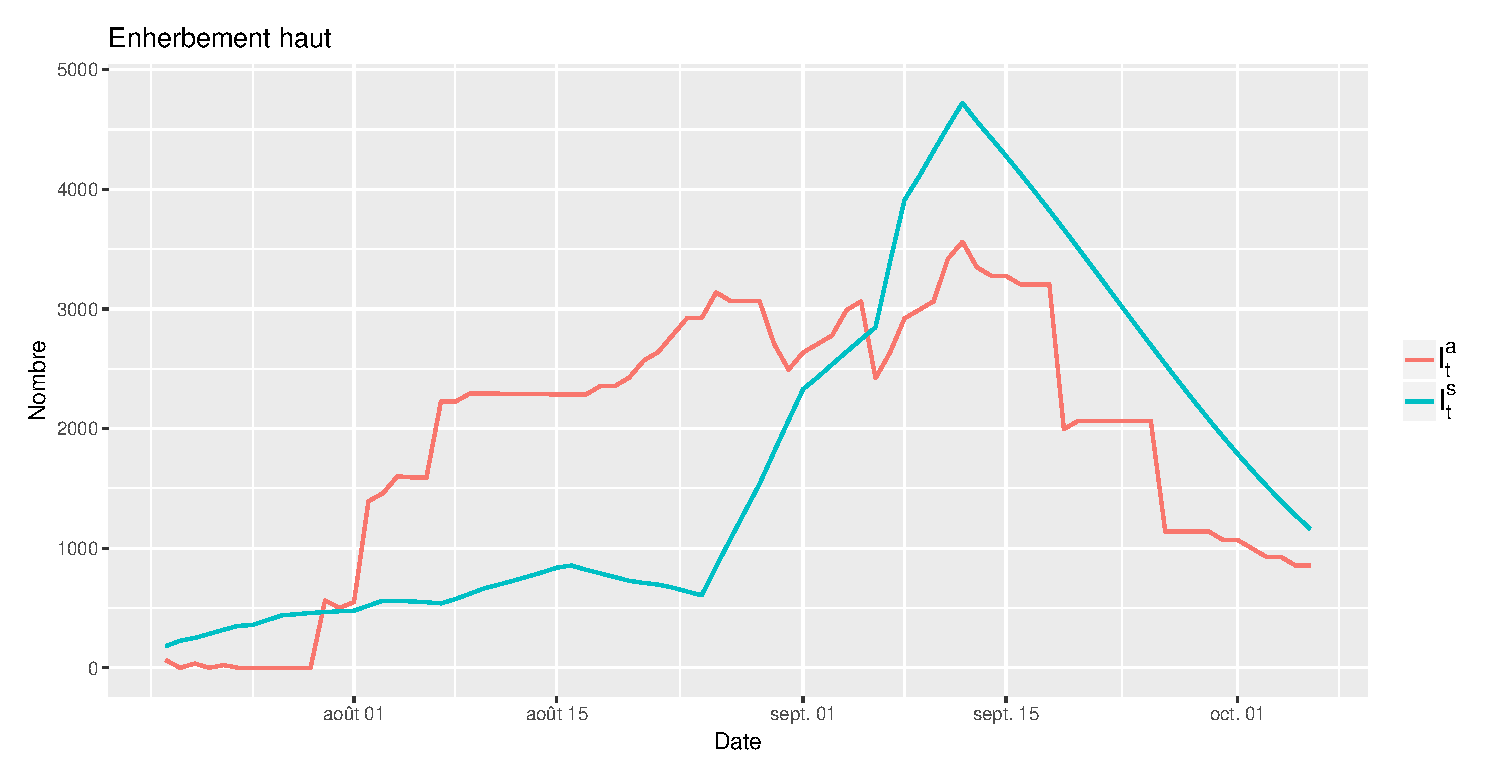
\epsfig{file = plots/comp_EH.eps, scale = 0.65}
\end{figure}

\newpage

Si pour les deux premiers sous-blocs les dynamiques semblent relativement similaires, le dernier sous-bloc montre des différences significatives entre les deux approches.

On peut également comparer la somme cumulée des dynamiques de débourrements entre les deux méthodes :

\begin{figure}[h]
 \centering
 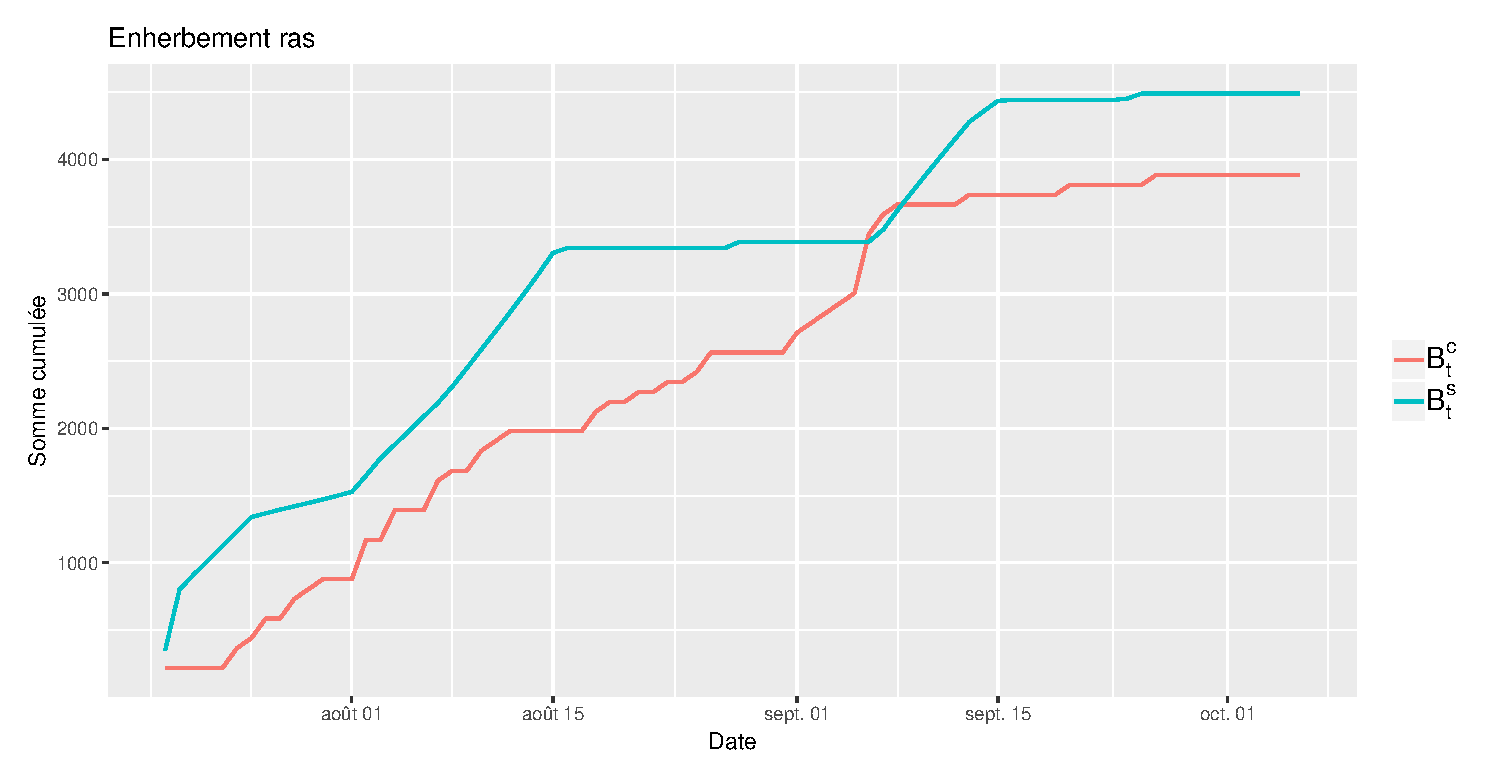
\epsfig{file = plots/comp_burst_ER.eps, scale = 0.65}
\end{figure}
 
\begin{figure}[h]
 \centering
 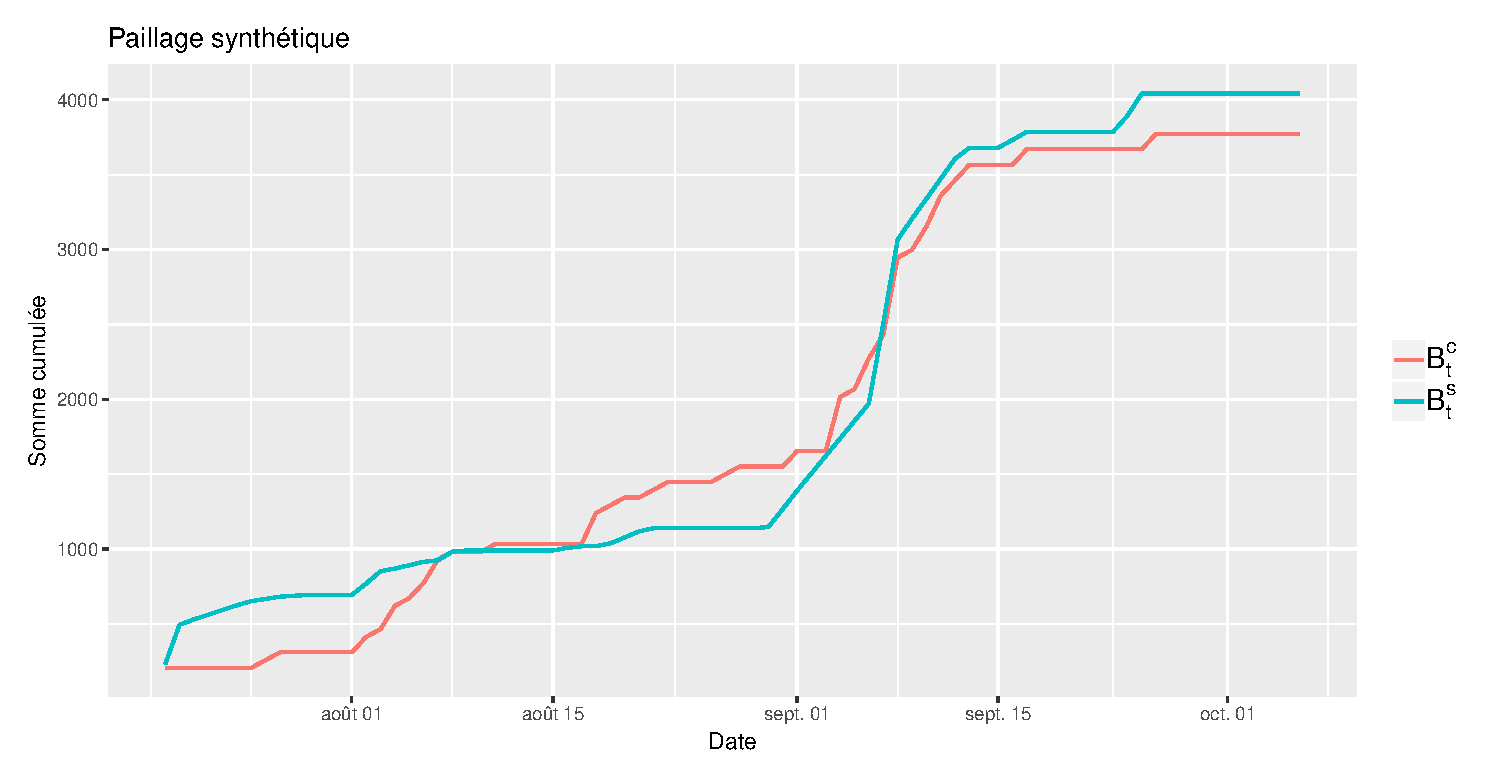
\epsfig{file = plots/comp_burst_PS.eps, scale = 0.65}
\end{figure}

\begin{figure}[ht]
 \centering
 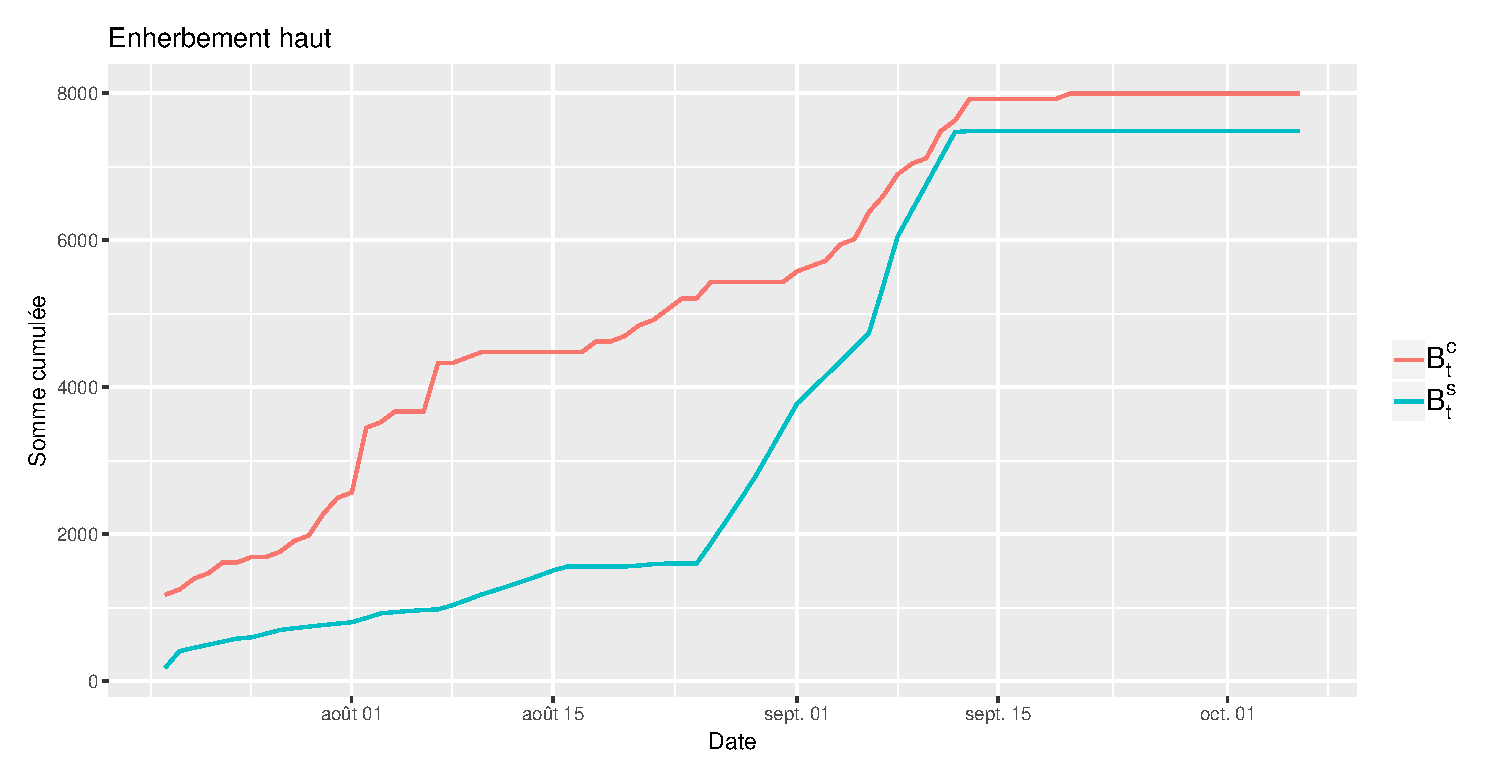
\epsfig{file = plots/comp_burst_EH.eps, scale = 0.65}
\end{figure}



\end{document}
